\documentclass[11pt,a4paper]{article}
\usepackage[margin=2.2cm]{geometry}
\usepackage[T1]{fontenc}
\usepackage{lmodern}
\usepackage{amsmath,amssymb}
\usepackage{graphicx}
\usepackage{booktabs}
\usepackage{caption}
\usepackage{subcaption}
\usepackage[hidelinks]{hyperref}
\usepackage{xcolor}
\captionsetup{font=small,labelfont=bf}
\graphicspath{{../figures/final/}{../figures/}}
\newcommand{\FNOrel}{0.0364}
\newcommand{\FNOstd}{0.0019}
\newcommand{\AdamState}{38.2}
\newcommand{\AdamPeakGPU}{4,043}
\newcommand{\ParamMB}{19.1}
\newcommand{\RsixteenRel}{0.0386}
\newcommand{\RsixteenState}{9.9}
\newcommand{\RfourState}{2.8}
\newcommand{\RfourRel}{0.0467}
\newcommand{\AdaHiRel}{0.0388}
\newcommand{\AdaHiEnd}{6.5}
\newcommand{\AdaHiPeak}{13.7}
\newcommand{\AdaHiMean}{7.8}
\newcommand{\AdaLoRel}{0.0454}
\newcommand{\AdaLoPeak}{4.6}
\newcommand{\AdaLoEnd}{2.6}
\newcommand{\PeakGPUlow}{3,956}
\newcommand{\PeakGPUhigh}{3,968}
\newcommand{\EnsAdam}{0.0310}
\newcommand{\EnsRsixteen}{0.0333}
\newcommand{\EnsGainLo}{14}
\newcommand{\EnsGainHi}{16}
\newcommand{\SpearLo}{0.55}
\newcommand{\SpearHi}{0.66}
\newcommand{\SpreadRatio}{0.74}
\newcommand{\KthreeRsixteenState}{29.6}
\newcommand{\KthreeRsixteenResident}{87}
\newcommand{\AdamResident}{57}
\newcommand{\SolverMean}{2.7e-05}
\newcommand{\SolverMax}{2.1e-04}
\newcommand{\SolverMedian}{1.7e-05}
\newcommand{\WrongSign}{0.86}
\newcommand{\NuThousand}{2.2e-02}
\newcommand{\NuFiveHundred}{2.2e-05}
\newcommand{\SpecLo}{0.85}
\newcommand{\SpecHi}{1.07}
\newcommand{\Grid256}{5.6e-06}
\newcommand{\FNOms}{3.48}
\newcommand{\SolThirtyTwoms}{0.30}
\newcommand{\SolThirtyTwoRel}{0.0326}
\newcommand{\SolThirtyTwoSpeed}{12}
\newcommand{\SolFortyEightms}{0.46}
\newcommand{\SolFortyEightRel}{0.0091}
\newcommand{\SolOneTwentyEightms}{15.5}
\newcommand{\SolOneTwentyEightSpeed}{4.4}
\newcommand{\BreakEvenFull}{145,377}
\newcommand{\TrainMin}{27}
\newcommand{\GenMin}{2.1}
\newcommand{\UnetMSE}{0.0555}
\newcommand{\UnetKtwo}{0.0516}
\newcommand{\BandMidMSE}{0.192}
\newcommand{\BandMidKtwo}{0.095}
\newcommand{\BandHighMSE}{34.5}
\newcommand{\BandHighKtwo}{3.8}
\newcommand{\ALgapLo}{4.1}
\newcommand{\ALgapHi}{6.2}
\newcommand{\ALstart}{0.0923}
\newcommand{\ALnMax}{3,000}
\newcommand{\ALnMin}{1,000}
\newcommand{\ALrandEnd}{0.0497}
\newcommand{\ALuncEnd}{0.0517}
\newcommand{\ALspearStart}{0.56}
\newcommand{\ALspearUncLo}{0.19}
\newcommand{\ALspearUncHi}{0.26}
\newcommand{\ALspearRandLo}{0.64}
\newcommand{\ALspearRandHi}{0.65}
\newcommand{\ALchosenLo}{1.3}
\newcommand{\ALchosenHi}{1.7}


\title{Rank-Adaptive Optimization for Memory-Efficient\\Neural Surrogates of Navier--Stokes Flow}
\author{Jay Gupta \and \textcolor{red}{[teammate names]}\\[2pt] \small FML Course Project}
\date{November 2026}

\begin{document}
\maketitle

\begin{abstract}
Adam stores two extra numbers per parameter; GaLore compresses each weight's gradient to a fixed low rank to
shrink this optimizer state. We ask whether choosing the rank \emph{adaptively} (per layer, per refresh, from the
gradient's energy spectrum) saves memory while keeping training quality, and whether the saving pays off for
ensembles of neural surrogates of a slow simulator. We implement a complex-aware low-rank Adam with fixed and
adaptive rank, verify it against \texttt{torch.optim.Adam}, and train Fourier Neural Operators (FNOs) that map a
forcing field to the vorticity of 2-D Navier--Stokes flow at $T=5$ (3 seeds per optimizer).
Low-rank optimizers cut FNO optimizer state from \AdamState\,MB to 2.6--9.9\,MB at the end of training (adaptive rank peaks at up to \AdaHiPeak\,MB during training) at a cost of 6--28\% in test error
(Adam \FNOrel; GaLore $r{=}16$ \RsixteenRel), but peak GPU memory falls by only about 2\% because activations dominate.
Adaptive rank lies on the same accuracy--memory curve as fixed rank and, once its \emph{peak} state during training
is counted, does not beat it. Three-member ensembles reduce error by \EnsGainLo--\EnsGainHi\% for every optimizer,
and member disagreement ranks test samples by error (Spearman \SpearLo--\SpearHi) but underestimates it.
We also wrote a pseudo-spectral solver that reproduces the dataset to a relative error of \SolverMean{}; on the same
GPU, a coarse $32^2$ solve matches the FNO's accuracy about \SolThirtyTwoSpeed$\times$ faster, so the surrogate offers no
speedup at matched accuracy for this problem.
\end{abstract}

% ======================================================================
\section{Problem}
Surrogates of slow simulators are often trained many times (ensembles for uncertainty, retraining as data
arrives). With Adam, each model carries an optimizer state twice the size of its parameters. GaLore~\cite{galore}
projects each weight's gradient onto its top-$r$ singular directions and keeps Adam's moments only in that
$r$-dimensional space, with one fixed $r$ for the whole run. The gradients of different layers, and of one layer at
different times, need not have the same effective rank. We test whether an adaptive rank does better than a fixed one
and measure what the memory saving buys in a surrogate workflow, including the surrogate's speed against the
simulator it replaces.

\paragraph{What is measured here.} Every number in this report is read from CSV files produced by the project
notebooks (\texttt{results/}); nothing is copied from the literature except where cited. Null and negative results
are reported as such.

% ======================================================================
\section{Data and its verification}
We use the \texttt{nsforcing\_128} dataset (Zenodo 12825163~\cite{zenodo}) from Kossaifi et~al.~\cite{mgtfno}:
10{,}000 training and 2{,}000 test pairs on a $128^2$ grid. The paper defines the problem as the vorticity equation
on the torus $[0,2\pi)^2$,
\begin{equation}
\partial_t \omega + u\cdot\nabla\omega = \nu\,\Delta\omega + f,\qquad u=\nabla^\perp\psi,\quad -\Delta\psi=\omega,
\qquad \omega(0)=0,
\end{equation}
with $\nu=1/500$ and the operator $f\mapsto\omega(T{=}5)$, forcing $f\sim\mathcal N(0,\,27(-\Delta+9I)^{-4})$. The
dataset's library docstring instead describes both fields as vorticity, and the time integrator, time step and native
grid are not stated. We therefore verified the reading ourselves (Fig.~\ref{fig:solver}):
\begin{itemize}\itemsep1pt
\item The input field's power per Fourier mode follows $c(|k|^2+9)^{-4}$ to within a factor \SpecLo--\SpecHi{} for
$1\le|k|\le 31$, as expected for the stated forcing.
\item Our pseudo-spectral solver (Sec.~\ref{sec:solver}) started from rest with $f=x$ and $\nu=1/500$ reproduces the
output field: on 50 test samples the relative $L^2$ error is \SolverMean{} on average (median \SolverMedian, max
\SolverMax). With $\nu=1/1000$ the error is \NuThousand; with the axes swapped it is \WrongSign.
On a $256^2$ grid the error drops to \Grid256, so the data were probably produced on a grid finer than $128^2$.
\end{itemize}
Solver settings were chosen on training samples; the test agreement was measured once afterwards.
So $x$ is the forcing and $y$ the vorticity at $T=5$. All models use the same 80/20 train/validation split
of the training file (seed 0) and train-set normalisation; the 2{,}000 test samples are used only for final
evaluation.

\begin{figure}[t]
\centering
\begin{subfigure}{0.36\linewidth}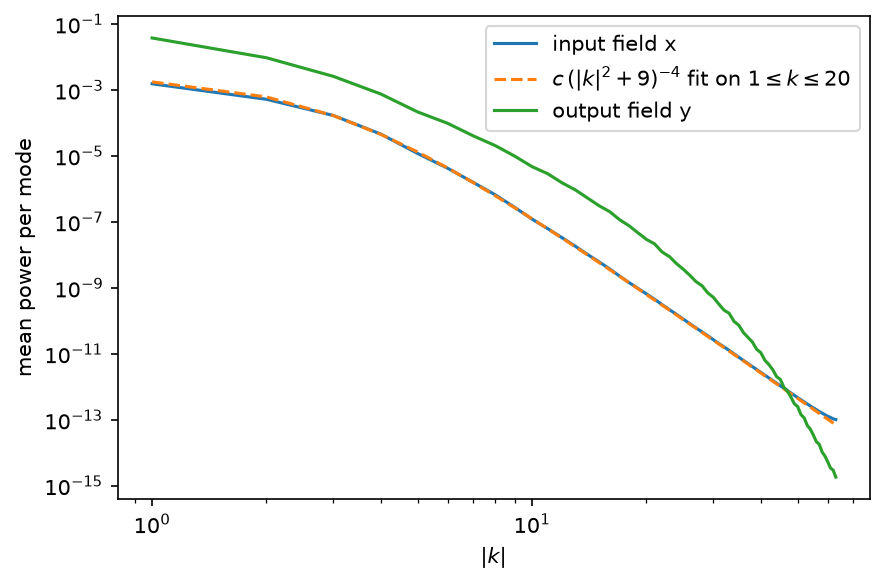
\includegraphics[width=\linewidth]{stage4_input_spectrum.png}\caption{}\end{subfigure}
\hfill
\begin{subfigure}{0.62\linewidth}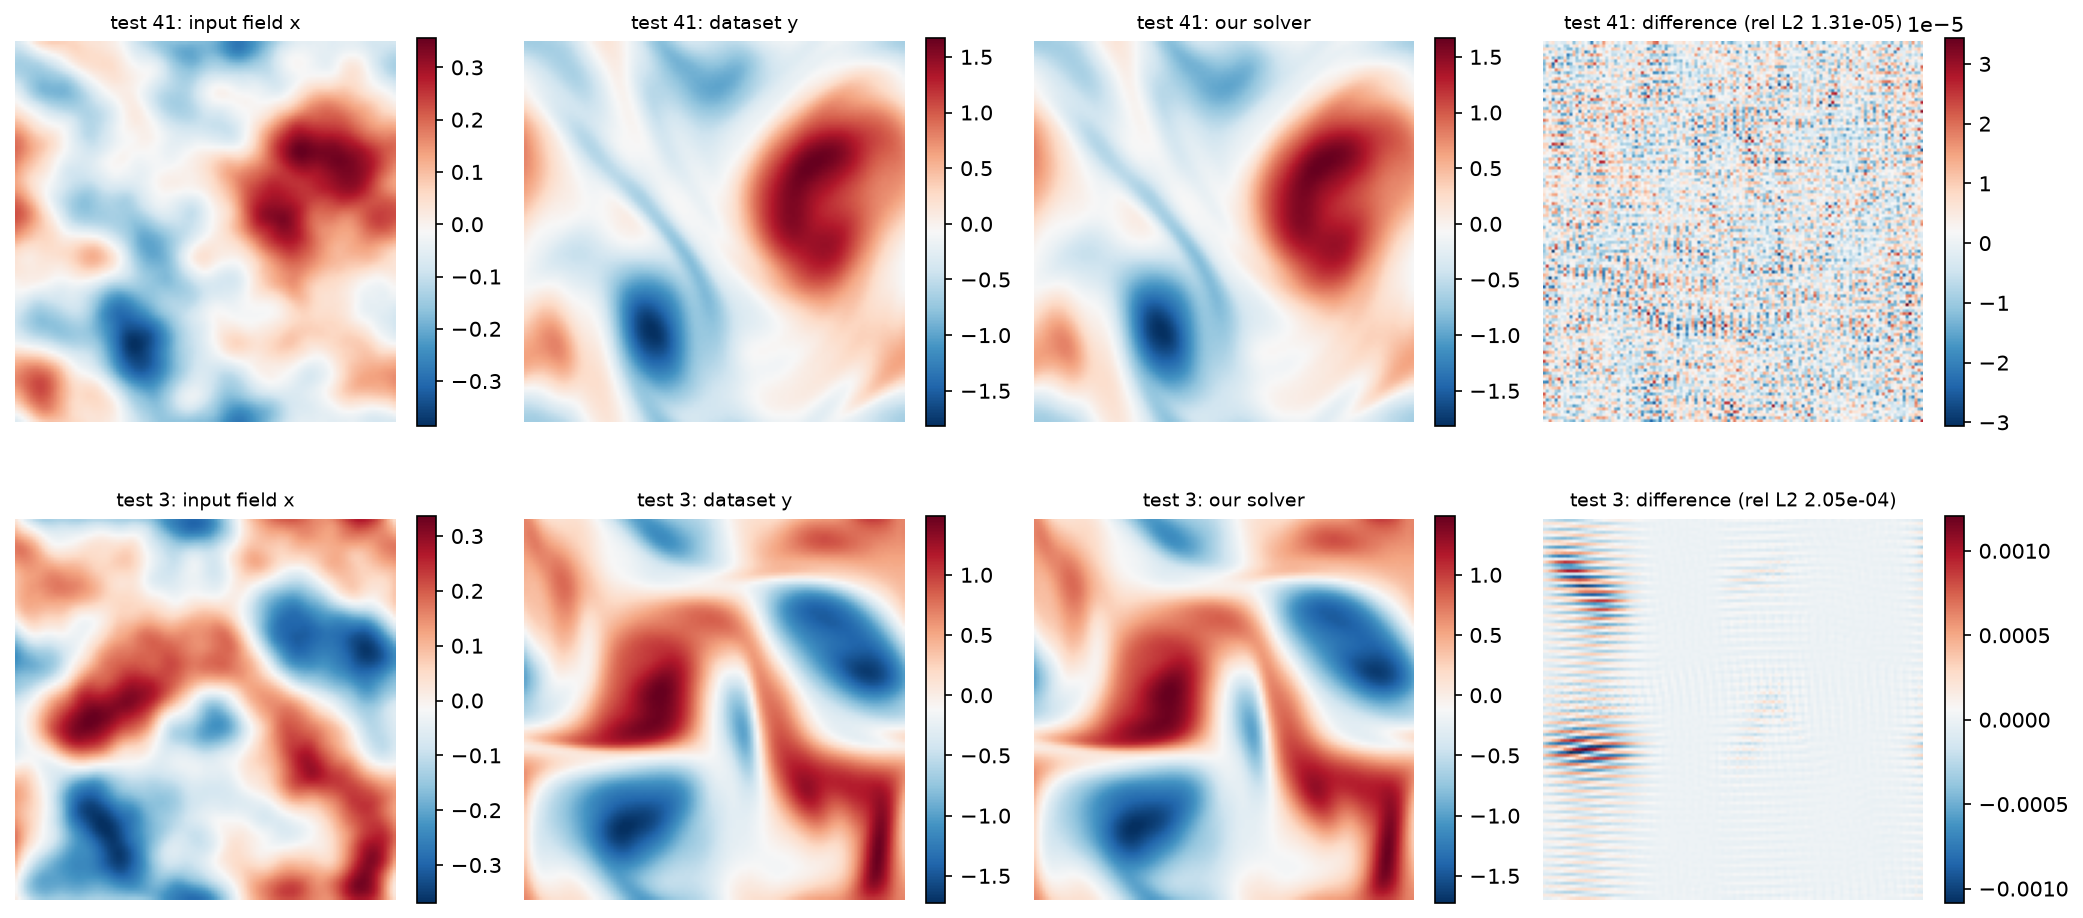
\includegraphics[width=\linewidth]{stage4_examples.png}\caption{}\end{subfigure}
\caption{Dataset verification. (a) Power per mode of the input field against the stated forcing covariance.
(b) Test samples with the smallest (top) and largest (bottom) disagreement between our solver and the dataset.}
\label{fig:solver}
\end{figure}

% ======================================================================
\section{Methods}
\subsection{Surrogates}
\textbf{FNO}~\cite{fno} (\texttt{neuraloperator}): 4 Fourier layers, 64 channels, $16\times16$ retained modes,
2{,}410{,}177 parameters. Its four spectral weights are complex tensors of shape $64\times64\times16\times9$ and hold
97.9\% of the parameters. \textbf{U-Net}~\cite{unet} (base width 32, 2{,}140{,}065 parameters) is the convolutional
baseline. Models are trained with MSE on standardised fields; for the U-Net we also test an $H^1$-type spectral loss
\[
\mathcal L = \mathrm{MSE}(\hat y,y) + \lambda\,\frac{\sum_k |k|^2\,|\hat Y_k - Y_k|^2}{\sum_k |k|^2\,|Y_k|^2},\qquad \lambda=0.5,
\]
with $\hat Y, Y$ the 2-D Fourier transforms of prediction and target (sums over modes and the batch).

\subsection{Low-rank Adam with fixed or adaptive rank}
For a weight with gradient reshaped to $G\in\mathbb{C}^{m\times n}$ (for the FNO, $m=64$, $n=64\cdot16\cdot9=9216$),
we keep an orthonormal basis $P\in\mathbb{C}^{m\times r}$ of the top-$r$ left singular vectors of $G$, refreshed
every 200 steps, run Adam on the projected gradient $R=P^{H}G\in\mathbb{C}^{r\times n}$, and apply the update
$P\,\mathrm{Adam}(R)$. $P$ comes from the eigen-decomposition of the small matrix $GG^{H}$. Complex numbers are
handled exactly as \texttt{torch.optim.Adam} does (moments on real and imaginary parts). Moments are kept when the
basis is refreshed (zero-padded or truncated when $r$ changes), as in the original GaLore.
\begin{itemize}\itemsep1pt
\item \textbf{Fixed rank} (GaLore): $r\in\{4,8,16\}$.
\item \textbf{Adaptive rank}: at each refresh, $r$ is the smallest $k$ whose cumulative gradient energy
$\sum_{i\le k}\sigma_i^2/\sum_i\sigma_i^2$ reaches $\tau$, with the normalised spectrum smoothed over refreshes
and $r\in[2,64]$; $\tau\in\{0.95,0.99,0.999\}$.
\end{itemize}
Only the four spectral weights are compressed; the remaining 2\% of parameters use ordinary Adam.
Optimizer-state memory counts every tensor the optimizer keeps (moments, $P$, smoothed spectrum).
For adaptive rank we report both the state at the end of training and its \emph{peak} during training, computed
from the logged ranks; the formula reproduces the measured state of the fixed-rank runs exactly.

\paragraph{Correctness.} 27 unit tests: with an identity basis the optimizer reproduces \texttt{torch.optim.Adam}
to $10^{-12}$ for real and complex tensors of both orientations; state shapes, memory, rank selection on
gradients of known rank, all basis-change modes and the refresh schedule are checked. A gradient study on the
original training run found that the four spectral-weight gradients reach 95\% of their energy with ranks of only
2.0, 3.6, 4.1 and 4.7 (of 64; averaged over 3{,}000 steps), which motivates both low rank and a per-layer rank.

\subsection{Ensembles}
$K=3$ FNOs per optimizer (seeds 0--2). The prediction is the member mean; uncertainty is the per-sample member
spread (standard deviation) relative to the target norm.

\subsection{Reference solver}\label{sec:solver}
Batched pseudo-spectral solver in PyTorch (CPU or GPU): exact spectral derivatives, 2/3-rule de-aliasing,
Crank--Nicolson diffusion with Heun's method for advection and forcing. Ten unit tests check exact
decay of Laplacian eigenmodes, the forced steady-mode solution, the expected convergence orders (1, 2 and 4
for the three implemented steppers) and batching. Coarse solves truncate the forcing to the grid and zero-pad
the output back to $128^2$.

\subsection{Protocol}
All FNO runs: lr $10^{-3}$, batch 32, 20 epochs (250 steps per epoch), MSE, best epoch by validation loss, 3 seeds,
identical data and initialisation per seed. Optimizer screening used 10 epochs and one seed; the finalists were then
trained in full. Every optimizer uses the same learning rate (no per-optimizer tuning). Peak GPU memory and
optimizer-state memory are reported separately. Timing: Tesla T4, one warm-up call, CUDA synchronisation around each
timed call, median of three repeats, best throughput over batch sizes 1, 32 and 256.

% ======================================================================
\section{Results}
\subsection{Baselines}
\begin{table}[h]
\centering\small\begin{tabular}{lccc}
\toprule
run & selection & best epoch & test rel.\ $L^2$ \\
\midrule
U-Net MSE, lr $0.001$ & val.\ MSE 0.0034 & 20 & 0.0555 \\
U-Net MSE, lr $0.0003$ & val.\ MSE 0.0050 & 19 & 0.0679 \\
U-Net MSE, lr $0.0001$ & val.\ MSE 0.0113 & 20 & 0.1030 \\
U-Net spectral ($\lambda{=}0.5$, $|k|^2$), lr $0.001$ & -- & 20 & 0.0516 \\
FNO + Adam (3 seeds) & -- & -- & 0.0364 $\pm$ 0.0019 \\
\bottomrule
\end{tabular}
\caption{Baselines (test relative $L^2$, raw units). The U-Net learning rate was chosen by validation MSE; the
spectral loss was then trained at the same rate. U-Net rows are single runs.}
\label{tab:baselines}
\end{table}
The FNO is the strongest surrogate (\FNOrel{}$\,\pm\,$\FNOstd, Table~\ref{tab:baselines}). For the U-Net, the
spectral loss lowers test error from \UnetMSE{} to \UnetKtwo; by frequency band, it halves the mid-band
($8\le k\le32$) relative error energy (\BandMidMSE$\to$\BandMidKtwo) and cuts spurious high-frequency
($k>32$) error energy from \BandHighMSE{} to \BandHighKtwo{} times the true energy there (Fig.~\ref{fig:bands}).
Low-band error is unchanged. This is one seed per loss, and the overall difference is within the
seed-to-seed spread seen for the FNO, so we read it as a change in \emph{where} the error lies rather than a
clear overall gain.

\begin{figure}[t]
\centering
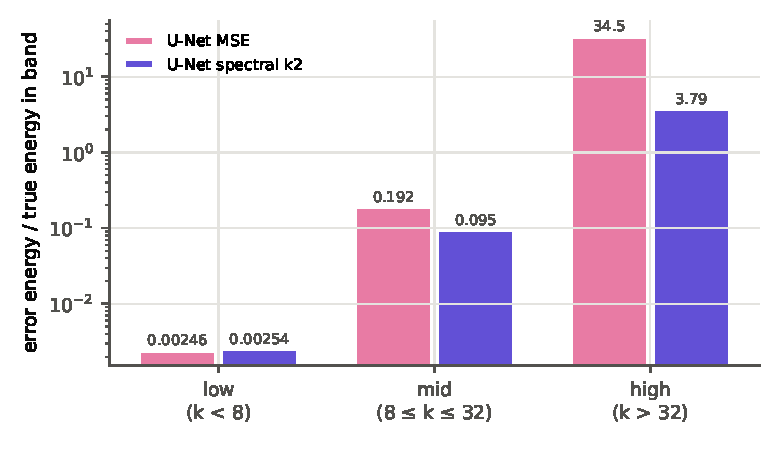
\includegraphics[width=0.55\linewidth]{fig_unet_bands.pdf}
\caption{U-Net test error energy divided by true energy, per frequency band, for MSE and spectral-loss training.}
\label{fig:bands}
\end{figure}

\subsection{Optimizers: memory and accuracy}
\begin{table}[t]
\centering\small\begin{tabular}{lcccccc}
\toprule
optimizer & test rel.\ $L^2$ & \multicolumn{2}{c}{optimizer state (MB)} & peak GPU & s/epoch & $K{=}3$ ensemble \\
 & mean $\pm$ std & end & peak & (MB) & & test rel.\ $L^2$ \\
\midrule
Adam & 0.0364 $\pm$ 0.0019 & 38.2 & 38.2 & 4,043 & 81.1 & 0.0310 \\
GaLore $r{=}$16 & 0.0386 $\pm$ 0.0008 & 9.9 & 9.9 & 3,966 & 80.2 & 0.0333 \\
adaptive $\tau{=}$0.999 & 0.0388 $\pm$ 0.0003 & 6.5 & 13.7 & 3,968 & 81.7 & 0.0331 \\
GaLore $r{=}$8 & 0.0424 $\pm$ 0.0006 & 5.1 & 5.1 & 3,959 & 81.6 & 0.0361 \\
adaptive $\tau{=}$0.99 & 0.0454 $\pm$ 0.0013 & 2.6 & 4.6 & 3,958 & 79.6 & 0.0389 \\
GaLore $r{=}$4 & 0.0467 $\pm$ 0.0009 & 2.8 & 2.8 & 3,956 & 79.6 & 0.0394 \\
\bottomrule
\end{tabular}
\caption{FNO trained with each optimizer (20 epochs, 3 seeds). Optimizer state: at the end of training and peak
during training (equal for fixed rank and Adam). Last column: test error of the 3-seed ensemble.}
\label{tab:opt}
\end{table}

\begin{figure}[t]
\centering
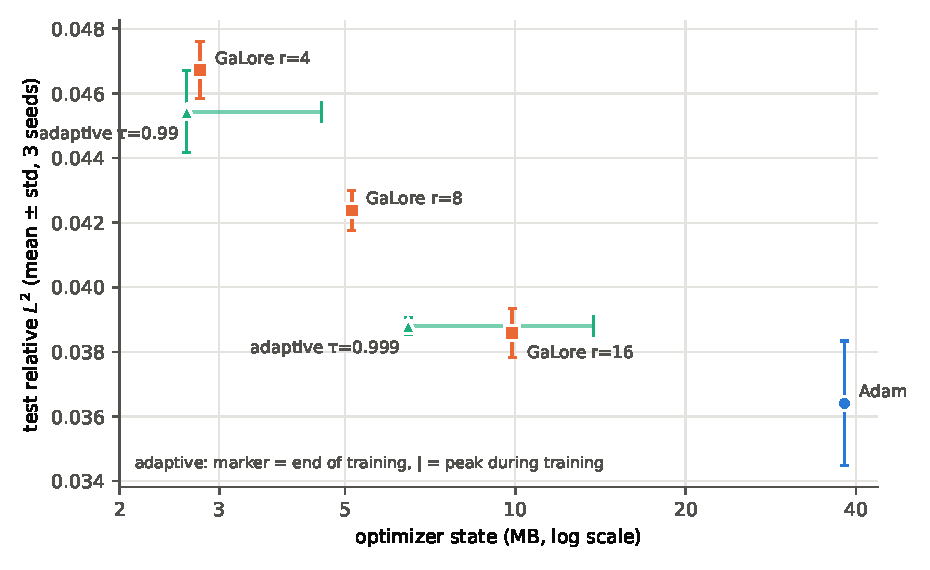
\includegraphics[width=0.62\linewidth]{fig_accuracy_vs_state.pdf}
\caption{Test error against optimizer-state memory (3 seeds). For adaptive rank the marker is the state at the end
of training and the bar extends to the peak state during training.}
\label{fig:pareto}
\end{figure}

Table~\ref{tab:opt} and Fig.~\ref{fig:pareto} give the main result.
\begin{itemize}\itemsep2pt
\item \textbf{State memory falls 4--15$\times$, peak GPU memory by about 2\%.} Adam keeps \AdamState\,MB of state;
GaLore $r{=}16$ keeps \RsixteenState\,MB and $r{=}4$ \RfourState\,MB. Peak GPU memory drops only from
\AdamPeakGPU{} to \PeakGPUlow--\PeakGPUhigh\,MB, because activations at batch 32 dominate it. Time per epoch is
unchanged (the projection costs little).
\item \textbf{Accuracy falls as state shrinks, but the gap narrows with training.} GaLore $r{=}16$ reaches
\RsixteenRel{} against Adam's \FNOrel{} (6\% higher); $r{=}4$ reaches \RfourRel{} (28\% higher). All low-rank runs
are still improving at epoch 20 (Fig.~\ref{fig:curves}), and the gap to Adam is smaller than after 10 epochs.
\item \textbf{Adaptive rank does not beat fixed rank.} Judged by end-of-training state, adaptive $\tau{=}0.999$
matches $r{=}16$ (\AdaHiRel{} vs \RsixteenRel) with \AdaHiEnd\,MB instead of \RsixteenState\,MB. But its rank is
highest early in training (Fig.~\ref{fig:rank}), so its peak state is \AdaHiPeak\,MB, more than $r{=}16$. Because
memory must be available at the peak, this is the relevant number. Adaptive $\tau{=}0.99$ against $r{=}4$
(\AdaLoRel{} vs \RfourRel) is within about one standard deviation. Adaptive rank lies on the same
accuracy--memory curve as fixed rank.
\item \textbf{The rank needed changes over training.} At $\tau{=}0.999$ the mean rank rises from 4 to about 19 in
the first two epochs and then falls to about 10 by epoch 20 (Fig.~\ref{fig:rank}). The early peak is what sets the
memory budget.
\end{itemize}

\begin{figure}[t]
\centering
\begin{subfigure}{0.49\linewidth}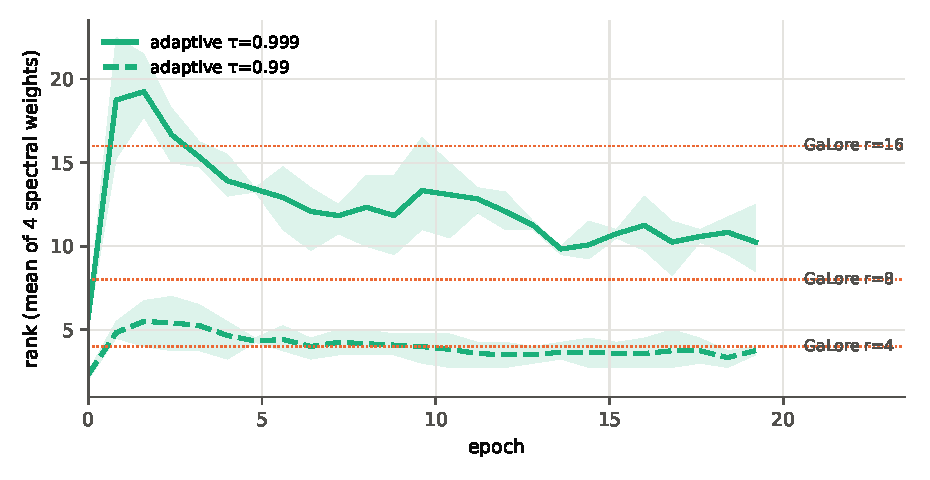
\includegraphics[width=\linewidth]{fig_adaptive_rank.pdf}\caption{}\label{fig:rank}\end{subfigure}
\hfill
\begin{subfigure}{0.49\linewidth}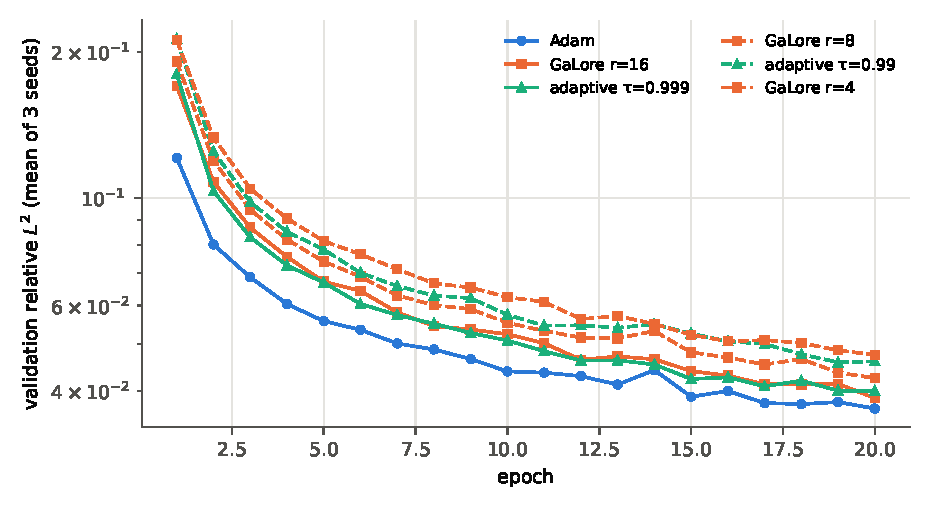
\includegraphics[width=\linewidth]{fig_val_curves.pdf}\caption{}\label{fig:curves}\end{subfigure}
\caption{(a) Rank chosen by the adaptive optimizer (mean of the four spectral weights; line = mean over 3 seeds,
band = range). (b) Validation error during training, mean of 3 seeds.}
\end{figure}

\subsection{Ensembles and uncertainty}
\begin{table}[h]
\centering\small\begin{tabular}{lcccc}
\toprule
optimizer ($K{=}3$) & mean member & ensemble & spread/error & Spearman \\
\midrule
Adam & 0.0364 & 0.0310 & 0.75 & 0.55 \\
GaLore $r{=}$16 & 0.0386 & 0.0333 & 0.70 & 0.55 \\
adaptive $\tau{=}$0.999 & 0.0388 & 0.0331 & 0.74 & 0.58 \\
GaLore $r{=}$8 & 0.0424 & 0.0361 & 0.74 & 0.61 \\
adaptive $\tau{=}$0.99 & 0.0454 & 0.0389 & 0.73 & 0.64 \\
GaLore $r{=}$4 & 0.0467 & 0.0394 & 0.78 & 0.66 \\
\bottomrule
\end{tabular}
\caption{Three-member ensembles. Spread/error: mean ratio of member spread to actual ensemble error per test
sample. Spearman: rank correlation between spread and error over the 2{,}000 test samples.}
\label{tab:ens}
\end{table}
Averaging three seeds lowers error by \EnsGainLo--\EnsGainHi\% for every optimizer (Table~\ref{tab:ens}). The spread
ranks samples by difficulty (Spearman \SpearLo--\SpearHi, Fig.~\ref{fig:spread}) but is on average only
\SpreadRatio{} of the actual error, so it is informative but not calibrated. For optimizer state alone, three
GaLore $r{=}16$ members need \KthreeRsixteenState\,MB, less than one Adam model (\AdamState\,MB), and their ensemble
(\EnsRsixteen) is more accurate than a single Adam model (\FNOrel). Counting the parameters themselves
(\ParamMB\,MB per FNO) the ensemble holds \KthreeRsixteenResident\,MB against \AdamResident\,MB for one Adam
model, and peak GPU memory per member is unchanged, so in this setting the memory saving does not by itself make
ensembles cheaper to hold.

\begin{figure}[t]
\centering
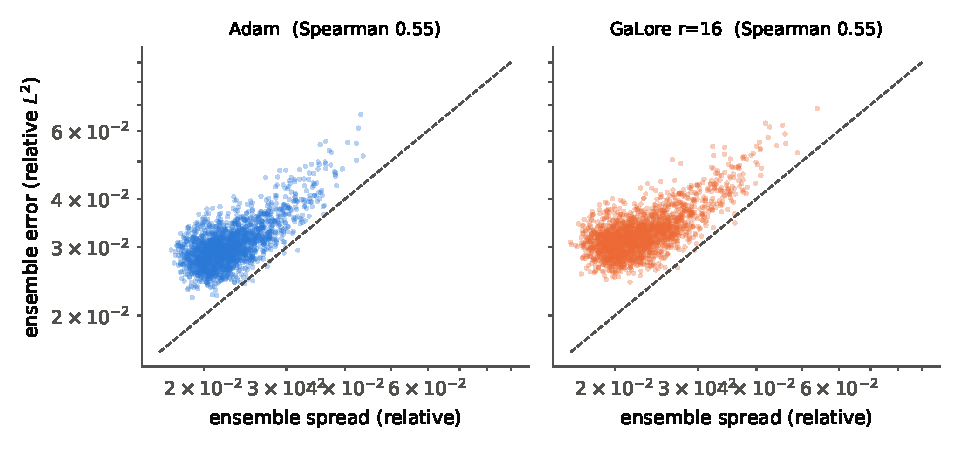
\includegraphics[width=0.7\linewidth]{fig_spread_error.pdf}
\caption{Ensemble spread against ensemble error per test sample. Dashed line: spread = error.}
\label{fig:spread}
\end{figure}

\subsection{Surrogate against the solver}
\begin{table}[t]
\centering\small\begin{tabular}{lccc}
\toprule
method & ms / sample & test rel.\ $L^2$ & FNO speedup \\
\midrule
solver $24^2$, $\Delta t=0.05$ & 0.30 & 7.8e-02 & 0.09$\times$ \\
solver $32^2$, $\Delta t=0.05$ & 0.30 & 3.3e-02 & 0.09$\times$ \\
solver $48^2$, $\Delta t=0.05$ & 0.46 & 9.1e-03 & 0.13$\times$ \\
solver $64^2$, $\Delta t=0.02$ & 2.53 & 2.3e-03 & 0.73$\times$ \\
solver $96^2$, $\Delta t=0.02$ & 5.77 & 3.0e-04 & 1.66$\times$ \\
solver $128^2$, $\Delta t=0.01$ & 15.49 & 4.2e-05 & 4.45$\times$ \\
solver $256^2$, $\Delta t=0.004$ & 192.62 & 3.2e-05 & 55.32$\times$ \\
FNO (single, Adam) & 3.48 & 0.0364 & -- \\
FNO, compile and autocast fp16 (seed 0) & 2.55 & 0.0378 & -- \\
FNO ($K{=}3$ ensemble) & 10.45 & 0.0310 & -- \\
\bottomrule
\end{tabular}
\caption{Time per sample on a Tesla T4 (best batch size) and test error against the dataset. Speedup = solver time /
FNO time; values below 1 mean the solver is faster.}
\label{tab:speed}
\end{table}

\begin{figure}[t]
\centering
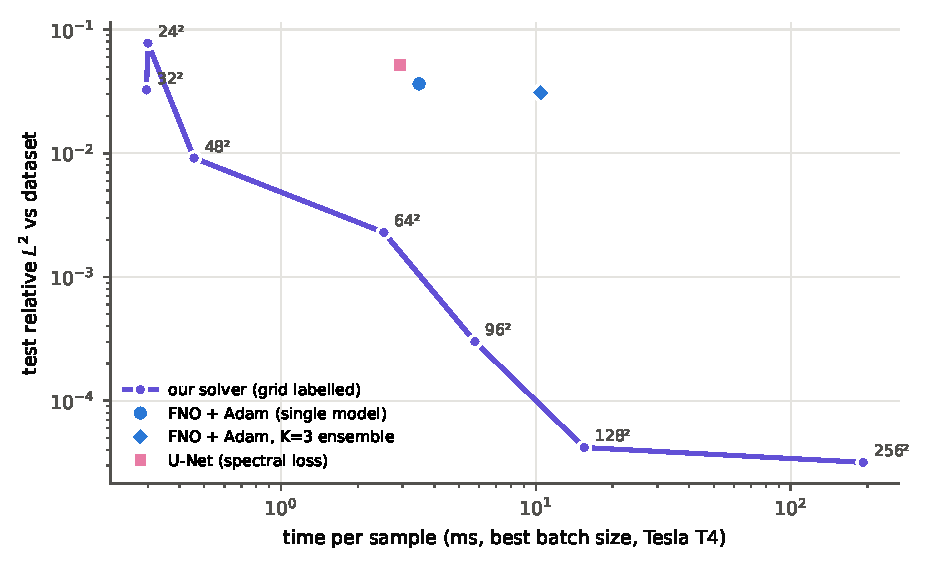
\includegraphics[width=0.62\linewidth]{fig_speed_accuracy.pdf}
\caption{Cost and accuracy of our solver on coarser grids (largest stable time step per grid), with the
surrogates, on the same GPU.}
\label{fig:speed}
\end{figure}
A surrogate's speedup must be judged against the cheapest solver setting with the same accuracy, not against a
fully resolved solve. Our solver on a $32^2$ grid with 100 time steps takes \SolThirtyTwoms\,ms per sample and
reaches \SolThirtyTwoRel, the same accuracy as the FNO (\FNOrel) at \FNOms\,ms, about \SolThirtyTwoSpeed$\times$
faster (Table~\ref{tab:speed}, Fig.~\ref{fig:speed}). A $48^2$ solve is four times more accurate than the FNO and
still faster. The FNO is \SolOneTwentyEightSpeed$\times$ faster than the $128^2$ solve, but that solve is
three orders of magnitude more accurate. Counting training (\TrainMin\,min) and generating 8{,}000 training samples
(\GenMin\,min), the FNO would need about \BreakEvenFull{} queries to pay off against the $128^2$ solver, and it never
pays off against a solver of matched accuracy. This holds for this smooth, moderately viscous flow over a short
horizon; harder regimes (higher Reynolds number, longer horizons) need finer grids and are where surrogates usually
gain.

% ======================================================================
\section{Limitations}
\begin{itemize}\itemsep1pt
\item One learning rate ($10^{-3}$, update scale 1) for every optimizer. GaLore is often run with a larger rate or
scale; the low-rank results may improve with tuning.
\item 20 epochs; the low-rank runs were still improving. Three seeds per optimizer; one seed per U-Net loss.
\item Memory: at this model size and batch, activations dominate peak memory. Larger models, smaller batches or
activation checkpointing would make optimizer state a larger share; we did not test them.
\item Ensembles of $K=3$ only. Planned active learning and multi-step rollout were not run within the time budget.
\item Timings are for one GPU type (T4) and float32; the FNO was not tried in lower precision.
\item The gradient-rank study comes from a single earlier training run.
\end{itemize}

\section{Conclusion}
A complex-aware low-rank Adam reduces FNO optimizer state 4--15$\times$ at a 6--28\% accuracy cost, and three such
models can be held for less optimizer state than one Adam model. An energy-threshold adaptive rank finds sensible,
layer-dependent ranks, but it reaches its largest rank early in training and, measured by peak memory, does no
better than a fixed rank. For this dataset the surrogate is also not faster than a coarse solve of equal accuracy.
These are null results, and they point to where adaptivity could help: a rank budget that bounds the early peak,
and problems where the optimizer state, not the activations, limits memory.

\begin{thebibliography}{9}\small
\bibitem{mgtfno} J.~Kossaifi, N.~Kovachki, K.~Azizzadenesheli, A.~Anandkumar. Multi-Grid Tensorized Fourier Neural
Operator for High-Resolution PDEs. arXiv:2310.00120, 2023.
\bibitem{zenodo} Navier--Stokes forcing dataset \texttt{nsforcing\_128}. Zenodo record 12825163.
\bibitem{galore} J.~Zhao, Z.~Zhang, B.~Chen, Z.~Wang, A.~Anandkumar, Y.~Tian. GaLore: Memory-Efficient LLM Training by
Gradient Low-Rank Projection. ICML 2024, arXiv:2403.03507.
\bibitem{fno} Z.~Li, N.~Kovachki, K.~Azizzadenesheli, B.~Liu, K.~Bhattacharya, A.~Stuart, A.~Anandkumar. Fourier
Neural Operator for Parametric Partial Differential Equations. ICLR 2021.
\bibitem{unet} O.~Ronneberger, P.~Fischer, T.~Brox. U-Net: Convolutional Networks for Biomedical Image Segmentation.
MICCAI 2015.
\bibitem{adam} D.~P.~Kingma, J.~Ba. Adam: A Method for Stochastic Optimization. ICLR 2015.
\bibitem{ens} B.~Lakshminarayanan, A.~Pritzel, C.~Blundell. Simple and Scalable Predictive Uncertainty Estimation
using Deep Ensembles. NeurIPS 2017.
\bibitem{ck} G.~J.~Chandler, R.~R.~Kerswell. Invariant recurrent solutions embedded in a turbulent two-dimensional
Kolmogorov flow. J.\ Fluid Mech.\ 722, 2013.
\end{thebibliography}

\appendix
\section{Reproducing}
Code: \texttt{nsbench/} (models, trainer, data), \texttt{optim/} (low-rank Adam), \texttt{solver/}; tests in
\texttt{tests/} (\texttt{python -m pytest tests}). One notebook per stage in \texttt{notebooks/}, built by
\texttt{tools/stage*\_notebooks.py}; GPU stages ran on Kaggle (Tesla T4), Stages 3--4 locally on CPU.
\texttt{tools/make\_final.py} rebuilds \texttt{results/FINAL.csv}, all report figures and every number in this
report from the stage CSVs.
\end{document}
